% Options for packages loaded elsewhere
\PassOptionsToPackage{unicode}{hyperref}
\PassOptionsToPackage{hyphens}{url}

  \PassOptionsToPackage{dvipsnames,svgnames,x11names}{xcolor}



%%%% Clase del documento y configuraciones generales de apariencia
\documentclass[
  %
  %
    a4paper,%
  %
  %
  %
    DIV=calc,%
  %
    abstract=true%
  ]{scrartcl}%

\usepackage{amsmath,amssymb}


\usepackage{iftex}

\ifPDFTeX                       % if pdflatex
  \usepackage[T1]{fontenc}
  \usepackage[utf8]{inputenc}
  \usepackage{textcomp}         % provide euro and other symbols
\else % if luatex or xetex
      \usepackage{unicode-math}   % this also loads fontspec
    \defaultfontfeatures{Scale=MatchLowercase}
  \defaultfontfeatures[\rmfamily]{Ligatures=TeX,Scale=1}
\fi

  
  \usepackage[]{Alegreya}

\ifPDFTeX\else    
  \usepackage{fontspec}
          
  
      \fi


\IfFileExists{upquote.sty}{\usepackage{upquote}}{}

\IfFileExists{microtype.sty}{
  \usepackage[]{microtype}
  \UseMicrotypeSet[protrusion]{basicmath} 
}{}

  \makeatletter
  \@ifundefined{KOMAClassName}{%    
    \IfFileExists{parskip.sty}{%
      \usepackage{parskip}
    }{
      \setlength{\parindent}{0pt}
      \setlength{\parskip}{6pt plus 2pt minus 1pt}}
  }{
    \KOMAoptions{parskip=half}}
  \makeatother


\usepackage{xcolor}





%%%% Configuración de tablas
  \usepackage{longtable,booktabs,array}
    \usepackage{calc} % for calculating minipage widths
  % Correct order of tables after \paragraph or \subparagraph
  \usepackage{etoolbox}
  \makeatletter
  \patchcmd\longtable{\par}{\if@noskipsec\mbox{}\fi\par}{}{}
  \makeatother
  % Allow footnotes in longtable head/foot
  \IfFileExists{footnotehyper.sty}{\usepackage{footnotehyper}}{\usepackage{footnote}}
  \makesavenoteenv{longtable}

%%%% Configuración de figuras
  \usepackage{graphicx}
  \makeatletter
  \def\maxwidth{\ifdim\Gin@nat@width>\linewidth\linewidth\else\Gin@nat@width\fi}
  \def\maxheight{\ifdim\Gin@nat@height>\textheight\textheight\else\Gin@nat@height\fi}
  \makeatother
  % Scale images if necessary, so that they will not overflow the page
  % margins by default, and it is still possible to overwrite the defaults
  % using explicit options in \includegraphics[width, height, ...]{}
  \setkeys{Gin}{width=\maxwidth,height=\maxheight,keepaspectratio}
  % Set default figure placement to htbp
  \makeatletter
  \def\fps@figure{htbp}
  \makeatother



\setlength{\emergencystretch}{3em} % prevent overfull lines
\providecommand{\tightlist}{%
  \setlength{\itemsep}{0pt}\setlength{\parskip}{0pt}}

  \setcounter{secnumdepth}{-\maxdimen} % remove section numbering




% Referencias con CSL
  % definitions for citeproc citations
  \NewDocumentCommand\citeproctext{}{}
  \NewDocumentCommand\citeproc{mm}{%
    \begingroup\def\citeproctext{#2}\cite{#1}\endgroup}
  \makeatletter
  % allow citations to break across lines
  \let\@cite@ofmt\@firstofone
  % avoid brackets around text for \cite:
    \def\@biblabel#1{}
    \def\@cite#1#2{{#1\if@tempswa , #2\fi}}
  \makeatother
  \newlength{\cslhangindent}
  \setlength{\cslhangindent}{1.5em}
  \newlength{\csllabelwidth}
  \setlength{\csllabelwidth}{3em}
  \newenvironment{CSLReferences}[2] % #1 hanging-indent, #2 entry-spacing
   {\begin{list}{}{%
    \setlength{\itemindent}{0pt}
    \setlength{\leftmargin}{0pt}
    \setlength{\parsep}{0pt}
    % turn on hanging indent if param 1 is 1
    \ifodd #1
      \setlength{\leftmargin}{\cslhangindent}
      \setlength{\itemindent}{-1\cslhangindent}
    \fi
    % set entry spacing
    \setlength{\itemsep}{#2\baselineskip}}}
  {\end{list}}
  \usepackage{calc}
  \newcommand{\CSLBlock}[1]{\hfill\break\parbox[t]{\linewidth}{\strut\ignorespaces#1\strut}}
  \newcommand{\CSLLeftMargin}[1]{\parbox[t]{\csllabelwidth}{\strut#1\strut}}
  \newcommand{\CSLRightInline}[1]{\parbox[t]{\linewidth - \csllabelwidth}{\strut#1\strut}}
  \newcommand{\CSLIndent}[1]{\hspace{\cslhangindent}#1}

  \ifLuaTeX
    \usepackage[bidi=basic]{babel}
  \else
    \usepackage[bidi=default]{babel}
  \fi
      \babelprovide[main,import]{spanish}
      
      \babelprovide[import]{english}
      % get rid of language-specific shorthands (see #6817):
  \let\LanguageShortHands\languageshorthands
  \def\languageshorthands#1{}


% Customizaciones generales %%%%%%%%%%%%%%%%%%%%%

%%%% CARGA DE PAQUETES
\usepackage[export]{adjustbox}

% Cargar paquetes de íconos 
\usepackage{fontawesome5}
\usepackage{ccicons}

% Carga `setspace' para separación entre lineas (si no fue cargado)
\IfPackageLoadedTF{setspace}{}{\usepackage{setspace}}
% Carga `graphicx' si no fue cargado (dado que no se usa entorno pandoc para figures)
\IfPackageLoadedTF{graphicx}{}{\usepackage{graphicx}}
% Carga `etoolbox' 
\IfPackageLoadedTF{etoolbox}{}{\usepackage{etoolbox}}

% Carga de paquetes y configuraciones pedidas por el documento
\IfPackageLoadedTF{tabularray}{}{\usepackage{tabularray}}

%%%% COLORES CUSTOMIZADOS

\definecolor{verde_orcid}{RGB}{166,206,57}

%%%% CITAS LARGAS

% Definir estilo de citas largas (achica el tamaño)
\IfPackageLoadedTF{relsize}{}{\usepackage{relsize}}
\AtBeginEnvironment{quote}{\smaller}% Step font down one size relative to current font.

%%%% TABLAS Y FGURAS

% Agregado de \source y \notes para titulos secundarios de las tablas y figuras
\usepackage{caption}
\captionsetup{format=plain,labelsep=period,singlelinecheck=false,justification=centerlast,
              font={small,singlespacing,sf},labelfont={sc,bf},width=0.8\textwidth}
\newcommand{\source}[1]{\vspace{-9pt}\caption*{\footnotesize{\textit{Fuente:} {#1}}}}
\newcommand{\notes}[1]{\vspace{-9pt}\caption*{\footnotesize{\textit{Notas:} {#1}}}}



% Cambia denominación de "Cuadro" a "Tabla"
\renewcommand{\spanishtablename}{Tabla}

% Cambiar fuente y tamaño de letra para entorno de tablas (table)
\AtBeginEnvironment{tabular}{\sffamily\footnotesize}
\IfPackageLoadedTF{tabularray}{%
\AtBeginEnvironment{tblr}{\sffamily\footnotesize}}{}

%%%% ENCABEZADO DE PÁGINA
% Si utiliza clases de Koma-script debe utilizar el paquete 'scrlayer-scrpage'
% Si utiliza las clases estándar debe usar el paquete 'fancyhdr'
\usepackage[headsepline]{scrlayer-scrpage}
\usepackage[breakwords]{truncate}

\setkomafont{pagehead}{\normalfont\sffamily\small}

\ihead{\textit{\truncate{0.45\textwidth}{Lorem ipsum}}}
\ohead{\textbf{\textasciitilde!guri\_ \{An example journal\}}}

\setkomafont{pagefoot}{\normalfont\footnotesize}
\ifoot[\rule{0.4\textwidth}{0.5pt} \vskip 0.5em Publicación de \emph{guri}.
      ISSN-e: 0001-2000.\\
      Esta obra está bajo una licencia Creative Commons
Attribution-NonCommercial-ShareAlike 4.0 International
License (https://creativecommons.org/licenses/by-nc/4.0/).]{}
\cfoot[]{\pagemark}

% Definir primera página del artícul (si se utiliza paginación personalizada)

%%%% PÁGINA DE TÍTULO 
\setkomafont{titlehead}{\raggedright\sffamily\small}
\setkomafont{title}{\raggedright\sffamily}
\setkomafont{author}{\raggedright\sffamily\setlength{\tabcolsep}{0pt}}
\setkomafont{publishers}{\raggedright\sffamily\footnotesize}
\setkomafont{dedication}{\raggedright\sffamily\small}

\titlehead{%
  \textbf\textbf{MODELO}\hfill\textbf{\textasciitilde!guri\_ \{An
example journal\}}\\%
  \vspace{4pt}
  \hfill Vol. 10 Núm. 1 (2023)
  \\ \hfill DOI: \href{https://doi.org/10.1223/3344445.55555333}{10.1223/3344445.55555333}%
 }%

\title{Lorem ipsum}

  \subtitle{Duis aute irure dolor\\ \vspace{1em} \textit{Pain itself}}

\author{{\begin{tabular}[l]{@{}l@{}}%
  \large{Marcus
Tullius {Cicero}}\textsuperscript{a;b} \href{https://orcid.org/0000-0000-1234-5678}{\textcolor{verde_orcid}{\faOrcid}}
\end{tabular}}%
}
    
\date{}

\publishers{
  \vspace{1em}
  \textsuperscript{a} Ancient
Rome, Italia.\\\textsuperscript{b} Platonic Academy, Grecia.
  \\ \vspace{1em} \textit{Recibido:} 1 de Septiembre de 2023; \textit{Aceptado:} 11 de Noviembre de 2023.\\%
}




%%% Credit, Ack and app Enviroment

\newenvironment{Credit}[1][Declaración de contribuciones de autoría (CRediT)]
    {\subsection*{#1}
    \sffamily\small}

\newenvironment{Ack}{\begin{Credit}[Agradecimiento]}{\end{Credit}}%

\newenvironment{app}{\newpage}{}
\ifLuaTeX
  \usepackage{selnolig}  % disable illegal ligatures
\fi






\usepackage{bookmark}

\IfFileExists{xurl.sty}{\usepackage{xurl}}{} % add URL line breaks if available
\urlstyle{same}



\hypersetup{
      pdftitle={Lorem ipsum},
        pdfauthor={Marcus Tullius Cicero},
    pdfsubject={\textasciitilde!guri\_ \{An example
journal\} - Volume: 10  - Issue: 1  (2023) a101 doi: 10.1223/3344445.55555333},
      pdflang={es-ES},
        pdfkeywords={Lorem, Ipsum, Dolor},
    pdfinfo={
          DOI={10.1223/3344445.55555333},
              abstract={Lorem ipsum dolor sit amet, consectetur
adipiscing elit, sed do eiusmod tempor incididunt ut labore et dolore
magna aliqua. Ut enim ad minim veniam, quis nostrud exercitation ullamco
laboris nisi ut aliquip ex ea commodo consequat. Duis aute irure dolor
in reprehenderit in voluptate velit esse cillum dolore eu fugiat nulla
pariatur. Excepteur sint occaecat cupidatat non proident, sunt in culpa
qui officia deserunt mollit anim id est laborum.},
        journal=\textasciitilde!guri\_ \{An example journal\}
      },
  % Define color de links
      colorlinks=true,
    linkcolor={CadetBlue},
    filecolor={CadetBlue},
    citecolor={CadetBlue},
    urlcolor={CadetBlue},
  pdfcreator={LaTeX via pandoc \& \textasciitilde!guri\_}}

%%%% Inicio de documento

\begin{document}
  
  
  \maketitle

  
    
    
    \begin{abstract}

      \noindent{Lorem ipsum dolor sit amet, consectetur adipiscing elit,
sed do eiusmod tempor incididunt ut labore et dolore magna aliqua. Ut
enim ad minim veniam, quis nostrud exercitation ullamco laboris nisi ut
aliquip ex ea commodo consequat. Duis aute irure dolor in reprehenderit
in voluptate velit esse cillum dolore eu fugiat nulla pariatur.
Excepteur sint occaecat cupidatat non proident, sunt in culpa qui
officia deserunt mollit anim id est laborum.}

      \nopagebreak

      \noindent\sffamily\textit{Palabras claves: Lorem; Ipsum; Dolor}.%

    \end{abstract}
    
        \begin{otherlanguage}{english}

      \begin{abstract}      
 
        \noindent{It is important to take care of the patient, to be
followed by the client, but at the same time they will be affected by
some great pains and sufferings. For to come to the smallest detail, no
one should practice any kind of work unless he derives some benefit from
it. Do not be angry with the pain in the rebuke, in the pleasure he
wants to be a hair from the pain, let him run away from the pain. Unless
they are blinded by lust, they do not come forth; they are in fault who
abandon their duties and soften their hearts, that is, their labors.}

        \nopagebreak

        \noindent\sffamily\textit{Keywords: Home; He himself; Pain}.%

      \end{abstract}
    \end{otherlanguage}
      

    
    
      
  
  
  \section{Dolor sit amet}\label{dolor-sit-amet}

  Lorem ipsum dolor sit amet, consectetur adipiscing elit. Mauris
  accumsan lectus non sem interdum condimentum. Nam at tincidunt sem. Ut
  cursus massa sagittis porta placerat. Sed consectetur diam est, ac
  sodales felis condimentum et. Fusce ut eros a massa molestie
  vestibulum. Donec blandit, augue non tempor laoreet, nisl velit cursus
  ante, vitae lobortis quam diam nec leo. In id nisi eget eros lobortis
  condimentum. Aenean a luctus quam. Mauris at vulputate nibh. Vivamus
  ultrices ligula velit, in volutpat tortor ullamcorper rhoncus:

  \begin{quote}
  Proin molestie enim est, et tempor est malesuada posuere. Nullam
  gravida, justo et aliquam fermentum, est dolor tincidunt arcu, vitae
  accumsan lectus eros et est. In laoreet est ut velit bibendum iaculis.
  Quisque et dignissim est, pharetra tempus diam.
  \end{quote}

  Pellentesque habitant morbi tristique senectus et netus et malesuada
  fames ac turpis egestas. Quisque eu ante tortor. Morbi vel tellus
  fringilla, ultrices nisi sit amet, ornare velit. Nunc rhoncus metus a
  massa venenatis mollis. Aliquam erat volutpat. Nam dui neque, aliquet
  a tempus eget, condimentum id libero. Ut tincidunt metus erat, eget
  feugiat nibh vestibulum nec. Maecenas nec quam a neque imperdiet
  bibendum eu eu risus. Pellentesque habitant morbi tristique senectus
  et netus et malesuada fames ac turpis egestas. Sed sed eros venenatis,
  consequat nunc eu, semper neque. Donec auctor facilisis metus et
  rhoncus. Vestibulum tempus tellus sed interdum posuere. Nulla bibendum
  fringilla nulla, sit amet tempus sem porttitor nec. Phasellus varius
  at tellus vitae sagittis. Ut rhoncus neque non est aliquet feugiat.
  Nullam condimentum luctus congue.

  \[E = \sqrt{p^{2}c^{2} + m^{2}c^{4} = mc^{2}}\]

  Phasellus ultricies nulla sed erat molestie mattis:
  \(P\left( \left. \ A \right|B \right) = \frac{P\left( \left. \ B \right|A \right)P(A)}{P(B)}\)
  . In congue tortor id venenatis luctus. Nulla a nulla vitae dolor
  porttitor porttitor quis sed urna. Curabitur at nisi et eros viverra
  porta quis eget neque. Donec at ante rhoncus, iaculis diam eget,
  egestas urna. Sed turpis tortor, facilisis vel neque eget, placerat
  bibendum leo. Mauris nec diam sed nisi cursus condimentum. Suspendisse
  suscipit turpis eu magna fringilla, id cursus tortor dignissim. Duis
  nisi lorem, facilisis id tincidunt ac, elementum quis risus.

  \section{Lorem ipsum}\label{lorem-ipsum}

  Mauris suscipit mattis lacinia. Donec a augue felis. Fusce imperdiet
  rutrum nibh, non elementum urna malesuada eu. Phasellus dolor mauris,
  molestie et augue a, luctus posuere quam. Nulla ut quam velit. Donec
  euismod, massa vitae tristique bibendum, metus lorem euismod lacus, id
  hendrerit enim nulla et lectus. Cras sit amet eros feugiat nibh
  ultricies luctus at et nisl. Nunc in tincidunt elit. Maecenas sit amet
  sem et justo fermentum pharetra. Duis venenatis aliquet arcu sed
  maximus. Suspendisse venenatis justo sed ipsum volutpat dictum. Duis
  dapibus, dui vel viverra semper, sapien metus placerat diam, non
  ornare dolor arcu quis massa. Nam ac rhoncus nisi.

  \begin{figure}
  \centering
  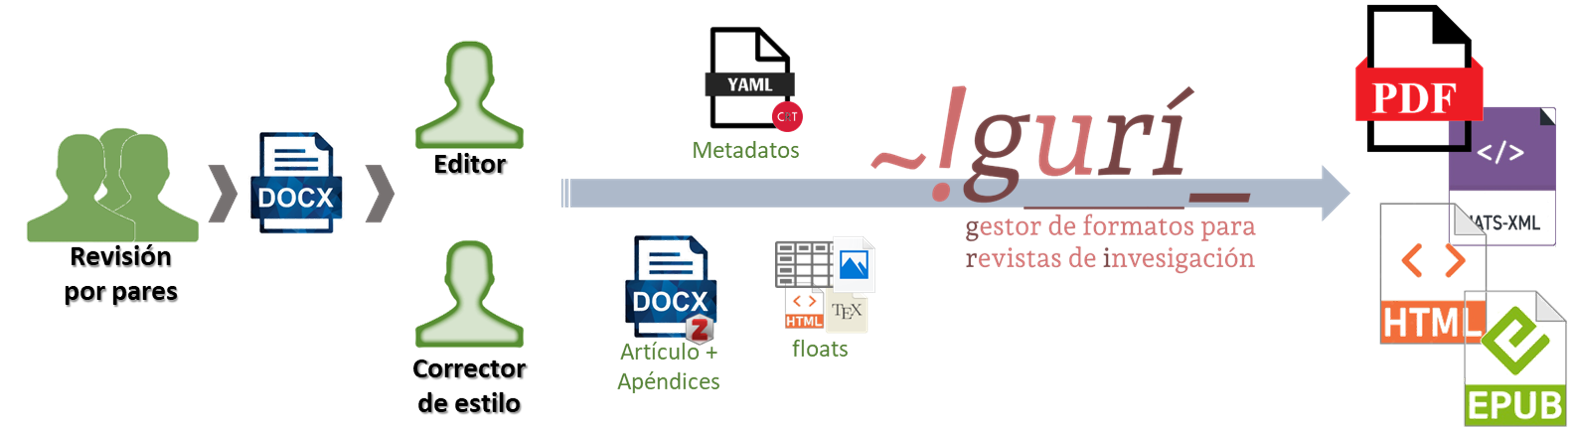
\includegraphics[width=0.9\textwidth]{./float/FIG_01}
  \caption{Lorem ipsum example}
  \source{Marcus Tullius Cicero (\citeproc{ref-27676}{1998, 45 BCE}).}
  \notes{Wikipedia says: “Lorem ipsum is typically a corrupted version of De finibus bonorum et malorum, a 1st-century BC text by the Roman statesman and philosopher Cicero, with words altered, added, and removed to make it nonsensical and improper Latin. The first two words themselves are a truncation of dolorem ipsum.”}
  \label{FIG_01}
  \end{figure}

  Etiam at maximus quam. Nam rhoncus, odio eu hendrerit iaculis, nisi
  massa gravida ante, eget tempor ante libero eget nisi. Donec fermentum
  diam tortor, ac tempor ex imperdiet tristique. Nam placerat lacinia
  arcu, sit amet auctor orci interdum eu. Maecenas sed tempus dui.
  Nullam imperdiet, arcu eget finibus dignissim, sapien diam feugiat
  lorem, at mattis metus sem a libero. Vestibulum vitae pretium risus.

  \subsection{Quis autem vel eum iure
  reprehenderit}\label{quis-autem-vel-eum-iure-reprehenderit}

  Quis autem vel eum iure reprehenderit, qui in ea voluptate velit esse,
  quam nihil molestiae consequatur, vel illum, qui dolorem eum fugiat,
  quo voluptas nulla pariatur? At vero eos et accusamus et iusto odio
  dignissimos ducimus, qui blanditiis praesentium voluptatum deleniti
  atque corrupti, quos dolores et quas molestias excepturi sint,
  obcaecati cupiditate non provident, similique sunt in culpa, qui
  officia deserunt mollitia animi, id est laborum et dolorum fuga
  (\hyperref[FIG_02]{Figura 2}).

  \begin{figure}
  \centering
  
\includegraphics[width=0.9\textwidth]{./float/FIG_02}
  \caption{Cicero's statue in the Capitoline Museums in Rome.}
  \source{Wikipedia (“Ciceron”).}
  \label{FIG_02}
  \end{figure}

  Fusce in nisl ut velit ornare malesuada. Etiam quis mauris vitae
  ligula pharetra condimentum ac ac orci. Curabitur aliquet justo nec
  quam posuere consectetur. Phasellus tincidunt rutrum lectus, eget
  viverra leo imperdiet sed. Aliquam vitae luctus mi. Maecenas a nulla
  elementum ipsum consequat scelerisque. Sed in mi pretium, pharetra
  odio ac, venenatis justo. Proin hendrerit mattis nisl, eu blandit
  libero cursus quis. Donec maximus volutpat arcu, quis laoreet purus
  mollis vel.

  \subsection{Praesent sollicitudin}\label{praesent-sollicitudin}

  Praesent sollicitudin lectus at eros rutrum aliquet. Aenean tempus
  ante a fermentum suscipit. Integer aliquet diam id elit pharetra, nec
  viverra ante faucibus. Nulla sit amet turpis enim. Vestibulum et
  pulvinar odio. Vestibulum euismod ante id placerat varius. Integer ac
  lacus nec felis sagittis elementum. Vestibulum arcu ipsum, eleifend eu
  eleifend eu, vestibulum in diam. Nunc interdum velit non tellus
  hendrerit vehicula. Aliquam sit amet justo ullamcorper leo tempor
  vulputate. Donec ultricies posuere odio, ac cursus odio mollis vel.
  Etiam nec gravida sapien.

  Sed condimentum diam orci, eget condimentum ipsum convallis quis. Sed
  ut perspiciatis, unde omnis iste natus error sit voluptatem
  accusantium doloremque laudantium, totam rem aperiam eaque ipsa
  \hyperref[TAB_01]{Tabla 1}, quae ab illo inventore veritatis et quasi
  architecto beatae vitae dicta sunt, explicabo.

  \begin{table}
  \caption{Frequency of occurrence of letters in common English and "Lorem Ipsum".}
  \label{TAB_01}
  \begin{tblr}{
      width = \linewidth,
      colspec = {Q[225]Q[315]Q[302]},
      column{1} = {c},
      column{3} = {c},
      hline{1-2,12} = {-}{0.08em},
  }
  \textbf{letter} & \textbf{English} & \textbf{Lorem} \\
  e               & 12.7 (1)         & 9.6 (1)        \\
  t               & 9.1 (2)          & 7.2 (5)        \\
  a               & 8.2 (3)          & 6.8 (2)        \\
  o               & 7.5 (4)          & 3.8 (7)        \\
  i               & 7 (5)            & 7.7 (13)       \\
  n               & 6.7 (6)          & 5.2 (3)        \\
  s               & 6.3 (7)          & 7.2 (6)        \\
  h               & 6.1 (8)          & 0.6 (11)       \\
  r               & 6 (9)            & 4.6 (9)        \\
  d               & 4.3 (10)         & 2.4 (14)       
  \end{tblr}
  \source{Own elaboration based on https://rpubs.com/kamerlingh/87951}
  \notes{The order of the letter in the frequency distribution is placed in brackets.}
  \end{table}

  \section{Praesent id nunc felis}\label{praesent-id-nunc-felis}

  Praesent id nunc felis. Aenean rutrum quam quis leo molestie, feugiat
  luctus arcu faucibus. Lorem ipsum dolor sit amet, consectetur
  adipiscing elit. Nullam mollis bibendum justo consequat pharetra.
  Mauris ornare eget erat eget varius. Phasellus lacinia congue justo.
  Sed malesuada et odio eget sodales. Etiam euismod tellus orci, lacinia
  consequat massa hendrerit elementum. Praesent dolor lacus, varius quis
  pharetra ut, lobortis in massa. Duis sit amet nunc ac nulla convallis
  viverra. Duis fermentum justo vitae erat condimentum convallis. Nam
  elementum orci vel lectus pulvinar, non mollis erat dignissim. Fusce
  volutpat auctor libero quis semper. Vivamus quam lorem, lobortis eget
  porta eget, volutpat vitae nibh.

  Nisi porta lorem mollis aliquam ut porttitor leo a diam.

  \begin{Credit}

  \phantomsection\label{Credit}
  \textbf{Cicero:} Conceptualización (Conceptualization); Curación de
  datos (Data curation); Análisis formal (Formal Analysis);
  Investigación (Investigation); Metodología (Methodology);
  Administración de proyecto (Project administration); Recursos
  (Resources); Redacción - preparación del borrador original (Writing --
  original draft); Redacción - revisión y edición (Writing -- review \&
  editing).

  \end{Credit}

  \begin{Ack}

  \phantomsection\label{Ack}
  Porta phasellus natoque fusce tempus aptent sem fames, mattis
  suspendisse inceptos ligula accumsan taciti.

  \end{Ack}

  \section{Referencias
  bibliográficas}\label{referencias-bibliogruxe1ficas}

  \phantomsection\label{refs}
  \begin{CSLReferences}{1}{0}
  \bibitem[\citeproctext]{ref-27676}
  Cicero, M. T. (1998). \emph{Cicero De Finibus Bonorum Et Malorum}.
  Clarendon Press.

  \end{CSLReferences}

  \begin{app}

  \phantomsection\label{app}
  \section{Appendix A: Some
  clarification}\label{appendix-a-some-clarification}

  Quis autem vel eum iure reprehenderit

  \section{Appendix B: Another thing}\label{appendix-b-another-thing}

  Maristella Igraine -- NGO 1, 24/04/2014.

  Hiba Dubgall -- NGO 2, 17/4/2014.

  Adebola Anaís -- NGO 3, 7/5/2014.

  Elias Audley -- Government, 4/5/2014.

  Clitus Laurus -- NGO 3, 16/04/2016.

  Santiago Rehoboam -- Government, 21/09/2016.

  Ana Mathildis, NGO 1, 19/03/2020.

  \end{app}

    
  %%%% Referencias bibliográficas
  
  
    
\end{document}
